\documentclass[oneside, 11pt]{article}

\usepackage[T1]{fontenc}
\usepackage[utf8]{inputenc}
\usepackage[dutch]{babel}

\usepackage{fouriernc}
\usepackage[detect-all, load-configurations=binary,
            separate-uncertainty=true, per-mode=symbol,
            retain-explicit-plus, range-phrase={ tot }]{siunitx}

\usepackage{setspace}
\setstretch{1.2}

\setlength{\parskip}{\smallskipamount}
\setlength{\parindent}{0pt}

\usepackage{geometry}
\geometry{marginparwidth=0.5cm, verbose, a4paper, tmargin=3cm, bmargin=3cm, lmargin=2cm, rmargin=2cm}

\usepackage{float}

\usepackage[fleqn]{amsmath}
\numberwithin{equation}{section}
\numberwithin{figure}{section}

\usepackage{graphicx}
\graphicspath{{Figures/}}
\usepackage{subfig}

\usepackage{tikz}
\usetikzlibrary{plotmarks}

\usepackage{fancyhdr}
\pagestyle{fancy}
\fancyhf{}
\rhead{\thepage}
\renewcommand{\footrulewidth}{0pt}
\renewcommand{\headrulewidth}{0pt}

\usepackage{relsize}
\usepackage{xspace}
\usepackage{url}

\newcommand{\figref}[1]{Figuur~\ref{#1}}

\newcommand{\hisparc}{\textsmaller{HiSPARC}\xspace}
\newcommand{\kascade}{\textsmaller{KASCADE}\xspace}
\newcommand{\sapphire}{\textsmaller{SAPPHiRE}\xspace}
\newcommand{\jsparc}{\textsmaller{jSparc}\xspace}
\newcommand{\hdf}{\textsmaller{HDF5}\xspace}
\newcommand{\aires}{\textsmaller{AIRES}\xspace}
\newcommand{\csv}{\textsmaller{CSV}\xspace}
\newcommand{\python}{\textsmaller{PYTHON}\xspace}
\newcommand{\corsika}{\textsmaller{CORSIKA}\xspace}
\newcommand{\labview}{\textsmaller{LabVIEW}\xspace}
\newcommand{\daq}{\textsmaller{DAQ}\xspace}
\newcommand{\adc}{\textsmaller{ADC}\xspace}
\newcommand{\adcs}{\textsmaller{ADC}s\xspace}
\newcommand{\Adcs}{A\textsmaller{DC}s\xspace}
\newcommand{\hi}{\textsc{h i}\xspace}
\newcommand{\hii}{\textsc{h ii}\xspace}
\newcommand{\mip}{\textsmaller{MIP}\xspace}
\newcommand{\hisparcii}{\textsmaller{HiSPARC II}\xspace}
\newcommand{\hisparciii}{\textsmaller{HiSPARC III}\xspace}
\newcommand{\pmt}{\textsmaller{PMT}\xspace}
\newcommand{\pmts}{\textsmaller{PMT}s\xspace}

\DeclareSIUnit{\electronvolt}{\ensuremath{\mathrm{e\!\!\:V}}}

\DeclareSIUnit{\unitsigma}{\ensuremath{\sigma}}
\DeclareSIUnit{\mip}{\textsmaller{MIP}}
\DeclareSIUnit{\adc}{\textsmaller{ADC}}

\DeclareSIUnit{\gauss}{G}
\DeclareSIUnit{\parsec}{pc}
\DeclareSIUnit{\year}{yr}



\title{\gps calibratie}
\author{A.P.L.S. de Laat}
\docdetector{3}{GC}
\version{1.0}

\begin{document}

\maketitle

\section{\gps bij \hisparc}\label{sec:gps_hisparc}

Bij \hisparc is het belangrijk dat we van ieder meetstation precies weten waar
het zich bevindt en op welk moment het iets meet. Voor zowel de
tijd als positie bepaling gebruiken we \gps. In dit document wordt
uitgelegd wat \gps is, waarom we het gebruiken, hoe de \gps bij een
\hisparc meetstations moet worden afgesteld en gekalibreerd en waarom we
voor bepaalde instellingen hebben gekozen.


\section{Het Global Positioning System}\label{sec:gps}

\gps staat voor Global Positioning System; een satelliet systeem voor
wereldwijde plaatsbepaling. Het bestaat uit een groep satellieten die
radiosignalen uitzendt waarmee het mogelijk is om wereldwijd te bepalen
waar je bent \cite{gps2013gov}. Het Amerikaanse project is in 1973
begonnen. De uitvinding van het systeem wordt toegekend aan Roger L.
Easton \cite{easton2006who}. Sinds 1994 is het systeem actief. \gps
bestaat momenteel uit 31 satellieten die in banen rond de aarde zijn
gebracht. In \figref{fig:GPSBlockIIIA} is een voorbeeld tekening van
zo'n \gps satelliet weergegeven. Elke \gps satelliet zit in een baan van
ongeveer \SI{20200}{\kilo\meter} boven de aarde. Elke satelliet cirkelt
in 12 uur om de aarde en zal daardoor (de aarde draait immers zelf ook)
elke 24 uur boven dezelfde plek op aarde zijn. Er zijn ook een aantal
tegenhangers van \gps ontwikkeld, namelijk het Russische GLONASS en het
Europese Galileo\footnote{Dit systeem is nog niet compleet, maar wordt
verwacht binnen een paar jaar operationeel te zijn.}. Tegenwoordig wordt
\gps door bijna iedereen gebruikt. Zo zitten er \gps ontvangers in onder
andere telefoons, auto's en ook de \hisparc elektronica.

\begin{figure}
    \centering
    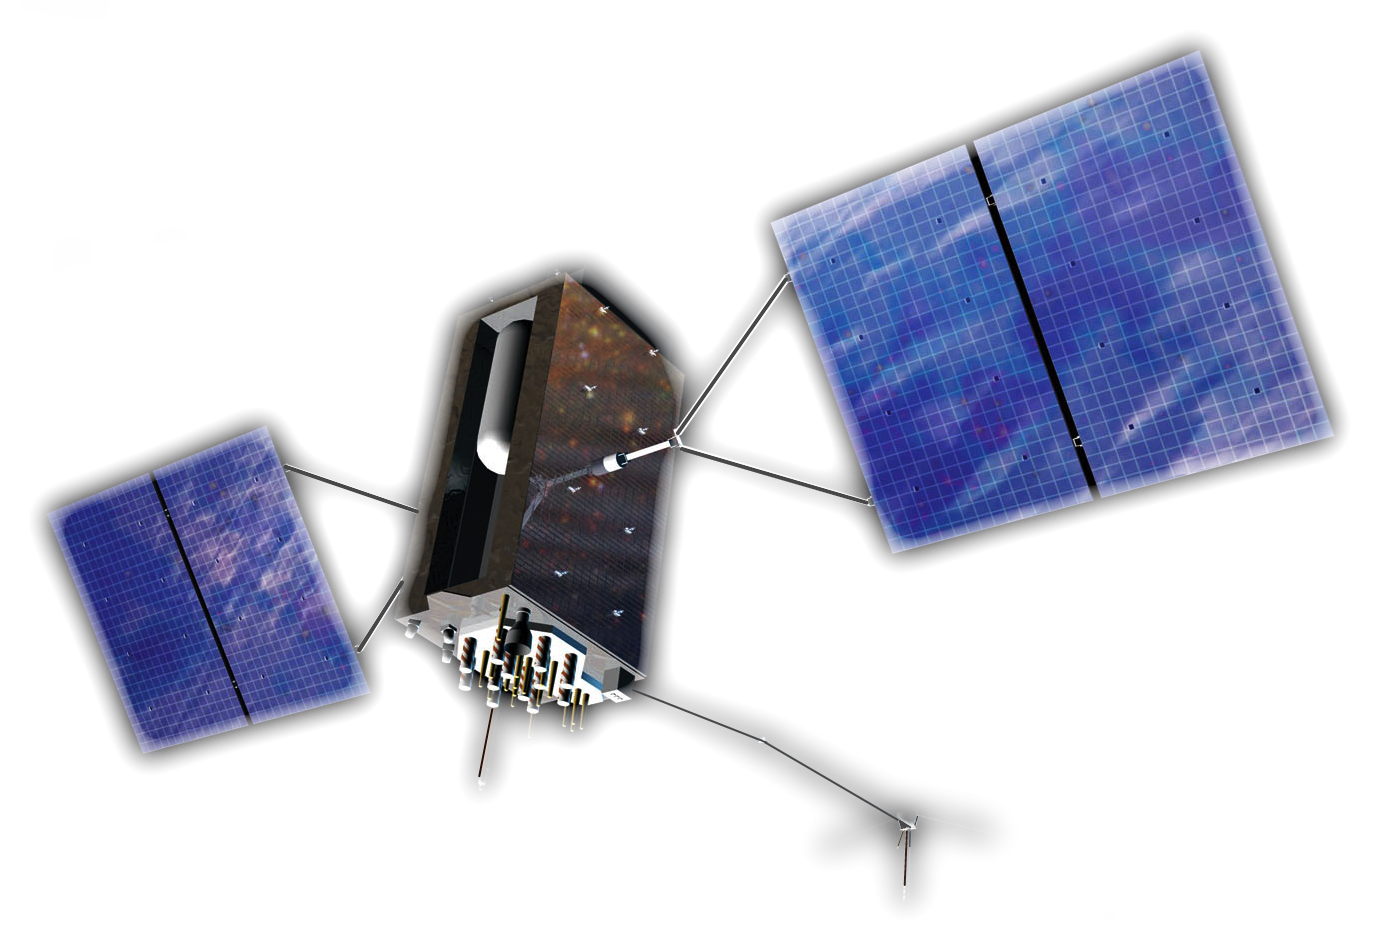
\includegraphics[scale=0.75]{GPS_Block_IIIA}
    \caption{Concept tekening van de volgende generatie \gps satellieten
    genaamd \gps Block IIIA. De eerste hiervan wordt in 2014 gelanceerd.
    Deze zullen een aantal nieuwe signalen uitzenden en meer zendkracht
    hebben. Dit moet leiden tot hogere nauwkeurigheid voor de gebruikers.}
    \label{fig:GPSBlockIIIA}
\end{figure}

\begin{figure}
    \centering
    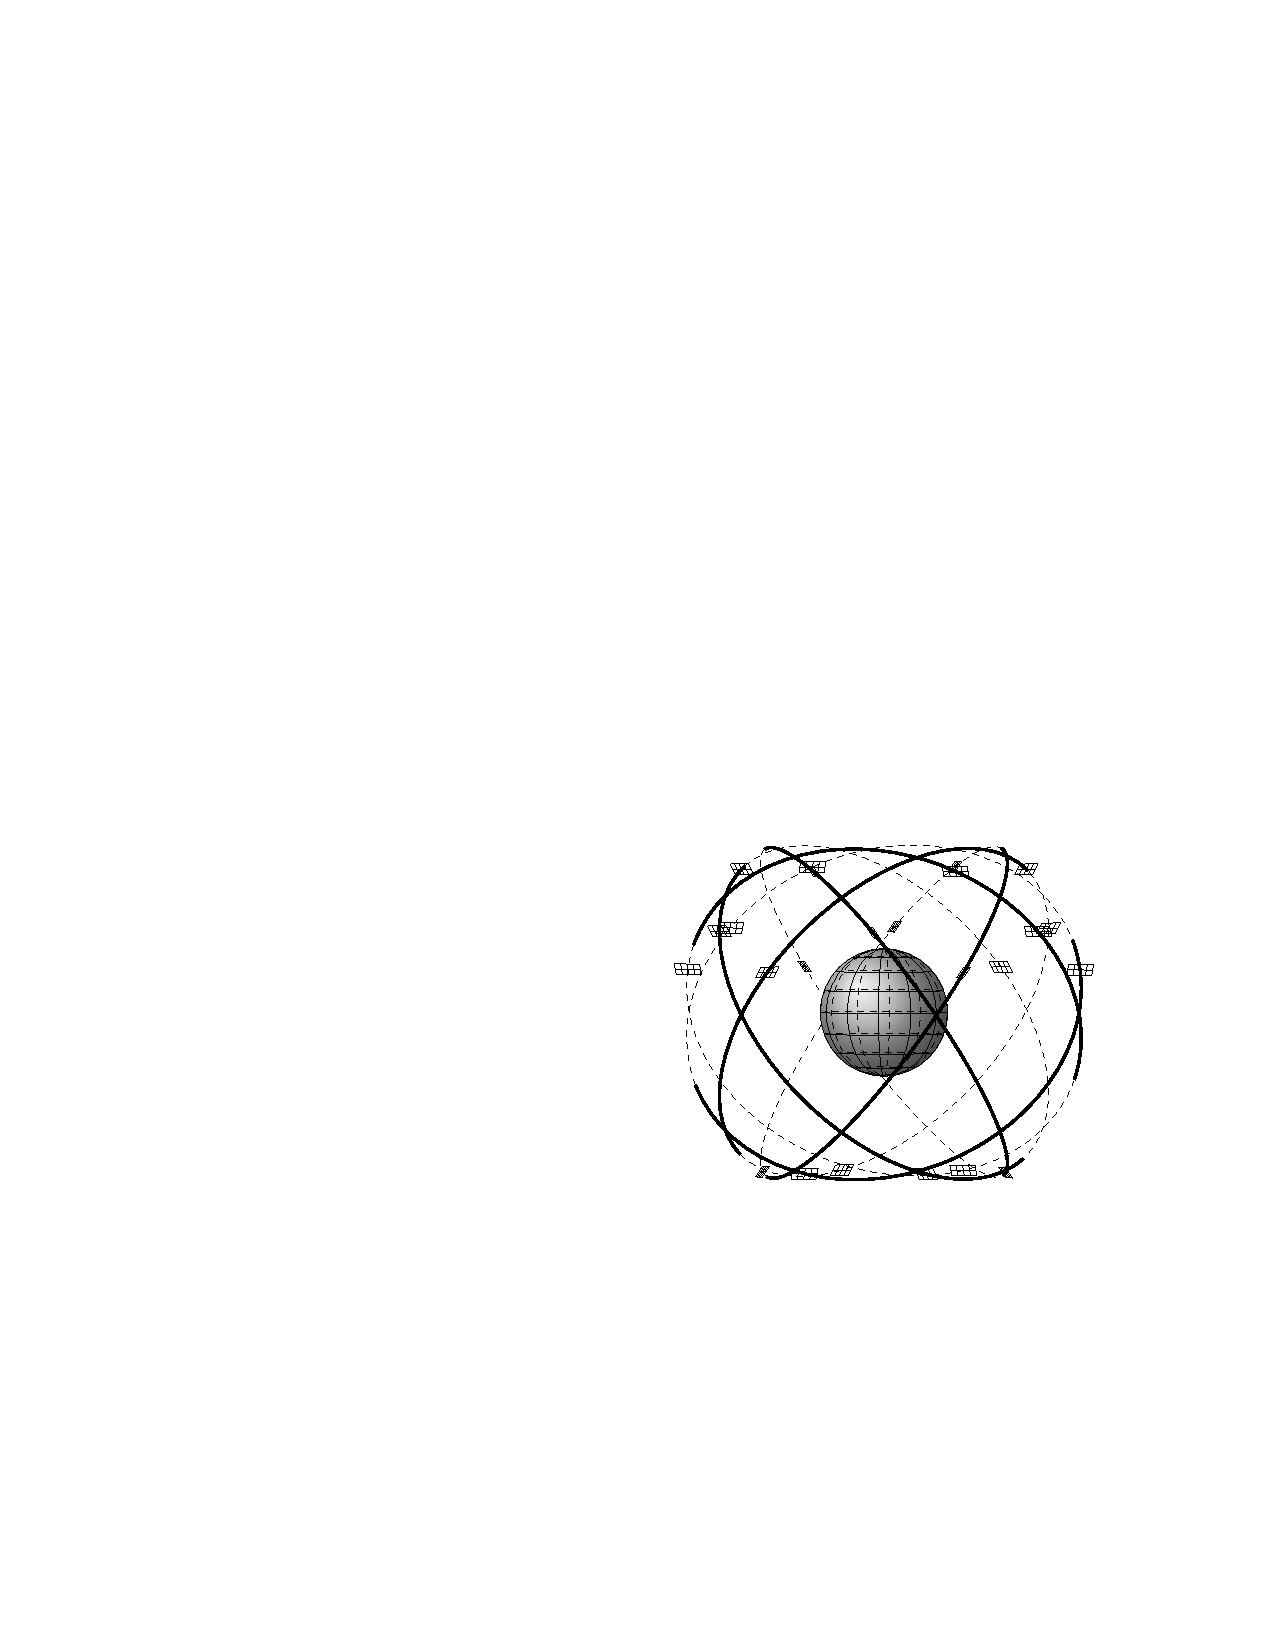
\includegraphics[scale=1]{GPS_satelliet_banen}
    % Thanks to: http://www.ux1.eiu.edu/~kwolcott/3DTikzGraphics.pdf
    \caption{Dit is een schematische weergave van de banen van de \gps
    satellieten rond de aarde. De satellieten zijn verdeeld over 6
    verschillende banen.}
    \label{fig:GPS_satelliet_banen}
\end{figure}


\section{Klokken}

Vroeger gebruikte men de zon en sterren om een ruwe schatting te maken
van de tijd \cite{gent2003wet}. Vanaf de dertiende eeuw werd er in
Europa gebruik gemaakt van mechanische uurwerken, maar deze waren zo
onnauwkeurig dat ze elke dag aan de hand van de stand van de zon moesten worden
bijgesteld. In 1656 werd door Christiaan Huygens het slingeruurwerk
uitgevonden. Deze was tot op een aantal seconden nauwkeurig over een
aantal dagen. Zo'n 10 jaar later ontwierp hij een klok met een
spiraalveer die in kleinere uurwerken gebruikt kon worden; zo kon men
ook een nauwkeurigere tijd bij zich dragen.

Het bijstellen van de openbare klokken werd binnen een stad vaak door
een lokale klokkenmaker gedaan; er was nog geen algemene tijd. Dit
betekende dat er tussen de meeste steden een tijdverschil was. Naarmate
de nauwkeurigheid van de klokken toenam werd het interessanter om betere tijd
afspraken te maken binnen een land. Zo werd in veel Europese landen de
middelbare zonnetijd gebruikt. In Nederland was daar nog weerstand tegen
omdat niet elke gemeente over de financiële middelen beschikte om de
nauwkeurigere klokken aan te schaffen.

Mogelijkheden voor snellere communicatie over langere afstanden
(telegraaf) en sneller reizen (spoorwegen) maakte het halverwege de
negentiende eeuw noodzakelijk om bijna overal in Nederland de middelbare
tijd van Amsterdam aan te houden. Toch was er nog lang onenigheid over
welke tijd precies aangehouden moest worden. Uiteindelijk werd in 1908
een wet aangenomen in Nederland, die stelde ''De wettelijke tijd in
Nederland is de middelbare zonnetijd van Amsterdam'' (Staatsblad
1908/236). Later kwamen er Europese en wereldwijde afspraken over
tijdzones, zomer- en wintertijd.

Tegenwoordig wordt de tijd bijgehouden door atoomklokken, uitgevonden door
de Amerikaanse National Institute of Standards and Technology (NIST).
Het NIST heeft een klok die zo nauwkeurig is dat het in 100 miljoen jaar
nog geen seconde verkeerd zal lopen \cite{nist2013ces}.

\gps doet niet mee aan zomer- en wintertijd, en ook niet aan de
schrikkelseconde\footnote{Een extra seconde die af en toe aan de tijd
wordt toegevoegd ter correctie van het verschil tussen de zonnedag en de
\SI{24}{uur} die als dag gezien wordt.}. Dit betekent dat de \gps
precies het aantal seconden sinds 1 January 1970 aangeeft. In het
verleden werkte \hisparc met UTC-tijd, maar dat had als nadeel dat
vanwege de schrikkelseconden een tijdstempel twee keer kon voorkomen.
Daarom wordt voor \hisparc nu gebruik gemaakt van \gps-tijd.


\section{Tijd en positie bepaling}

Bij \hisparc is het belangrijk dat we van ieder meetstation weten waar
het zich bevindt en precies op welk moment het iets meet. Deze gegevens
zijn namelijk nodig om te bepalen of verschillende meetstations dezelfde
shower hebben gemeten hebben en voor het uitvoeren van richting en
energie reconstructie. De meetstations liggen te ver uit elkaar om de
onderlinge posities met een meetlint en kompas te bepalen. Ook is het
niet mogelijk om de stations zo aan elkaar te koppelen dat hun klokken
tot op een aantal nanoseconden nauwkeurig gelijk staan.

Je eigen positie in 3 dimensies kun je bepalen als je de afstanden weet
ten opzichte van 3 bekende posities. Deze methode heet trilateratie. Je
zal dan namelijk 2 mogelijke posities vinden die precies die 3 afstanden
heeft tot de andere posities. Van deze twee posities is er maar \'e\'en
logisch.

Hieronder zijn de vergelijkingen te zien die horen bij de trilateratie
methode. Eerst voor 1, dan voor 2 en tenslotte voor 3 dimensies. Er komt
steeds een onbekende coördinaat bij. Omdat er ook steeds een
vergelijking bij komt is het stelsel vergelijkingen telkens op te
lossen. Voor het 1 dimensionale geval kun je veronderstellen dat je
ergens op een lijn staat, bijvoorbeeld de $x$-as. Jouw onbekende positie
is dan $x$. Als je de absolute afstand $d_1$ tussen jou en een ander
punt $x_1$ op dezelfde lijn weet, dan kan je $x$ vinden door de volgende
vergelijking op te lossen:
\begin{equation}
    \label{eq:1d_trilateratie}
    \begin{array}{rcl}
         d_1^2 = (x_1-x)^2 \\
    \end{array}
\end{equation}
Hier zijn twee oplossingen voor, namelijk $x = x_1+d_1$ en $x =
x_1-d_1$. In 2 dimensies komt er een tweede onbekende coördinaat bij,
$y$. Als je alleen de afstand $d_1$ tot een ander punt weet is de
oplossing voor $x$ en $y$ een cirkel met middelpunt $(x_1, y_1)$ en
straal $d_1$. De afstand $d_2$ tot een tweede punt $(x_2, y_2)$ is dus
noodzakelijk om je positie te bepalen. Dan onstaat het volgende stelsel
vergelijkingen:
\begin{equation}
    \label{eq:2d_trilateratie}
    \begin{array}{rcl}
         d_1^2 = (x_1-x)^2+(y_1-y)^2 \\
         d_2^2 = (x_2-x)^2+(y_2-y)^2 \\
    \end{array}
\end{equation}
Het stelsel heeft twee mogelijke oplossingen (de snijpunten van de twee cirkels).
In 3 dimensies willen we ook onze $z$ coördinaat bepalen. Het stelsel vergelijkingen wordt dan:
\begin{equation}
    \label{eq:trilateratie}
    \begin{array}{rcl}
         d_1^2 = (x_1-x)^2+(y_1-y)^2+(z_1-z)^2 \\
         d_2^2 = (x_2-x)^2+(y_2-y)^2+(z_2-z)^2 \\
         d_3^2 = (x_3-x)^2+(y_3-y)^2+(z_3-z)^2 \\
    \end{array}
\end{equation}
In deze 3 vergelijkingen zijn $x$, $y$ en $z$
de 3 onbekenden. Ook nu zijn er 2 mogelijke oplossingen (de snijpunten van 3 bollen). 

Bij \gps wordt, uiteraard, geen meetlint tussen de ontvanger en de
satelliet gespannen om achter de 3 benodigde afstanden te komen. In
plaats daarvan kijkt de ontvanger naar het tijdverschil tussen de tijd
waarop de \gps satelliet het signaal uitzendt en de tijd waarop hij dit
signaal ontvangt \cite{blewitt1997gps}. Als dit tijdverschil
vermenigvuldigd wordt met de lichtsnelheid (radiosignalen gaan met de
lichtsnelheid) heb je een afstand. De \gps satellieten zenden ook een
datapakket uit waarmee de posities van alle \gps satellieten op een
bepaalde tijd te bepalen valt. De positie van een \gps satelliet hangt
dus af van de tijd waarop een satelliet een signaal uitzend. Het is
echter nog onzeker of de tijd op de klok van de ontvanger correct is. Om
deze extra onbekende op te lossen is het signaal van een 4e satelliet
nodig. Het stelsel van vergelijkingen wordt daardoor als volgt:
\begin{equation}
    \label{eq:gps_stelsel}
    \begin{array}{rcl}
        d_1^2 = (c(t_{s,1}-t_{r,1}))^2 = (x_1-x)^2+(y_1-y)^2+(z_1-z)^2 \\
        d_2^2 = (c(t_{s,2}-t_{r,2}))^2 = (x_2-x)^2+(y_2-y)^2+(z_2-z)^2 \\
        d_3^2 = (c(t_{s,3}-t_{r,3}))^2 = (x_3-x)^2+(y_3-y)^2+(z_3-z)^2 \\
        d_4^2 = (c(t_{s,4}-t_{r,4}))^2 = (x_4-x)^2+(y_4-y)^2+(z_4-z)^2 \\
    \end{array}
\end{equation}
Eigenlijk volgen hier ook 2 mogelijke posities uit, maar meestal bevindt
de ontvanger zich op de Aarde, en zal de oplossing het dichtst bij de
Aarde is dan logischerwijs de correcte oplossing. Deze situatie is in 2D geschetst in
\figref{fig:Trilateratie}.

\begin{figure}
    \centering
    \includegraphics[scale=.6]{Trilateratie}
    \caption{Dit is een schematische weergave van trilateratie met \gps
             signalen. In dit voorbeeld is de $y$-as weggelaten. De
             satellieten ($S_{1,2}$) sturen signalen uit waar hun tijd
             en posities in zitten. De posities van de satellieten zijn
             dus bekend. De afstanden $d_{1,2}$ zijn te bepalen met
             behulp van het tijdverschil tussen $t_\textrm{verzonden}$ en
             $t_\textrm{ontvangst}$, als de tijd bij de ontvanger niet accuraat
             is is een extra satelliet nodig. Met deze afstanden zijn
             twee punten te vinden die die afstanden tot de satellieten
             hebben, maar er is er maar één op de Aarde!}
    \label{fig:Trilateratie}
\end{figure}


\section{Tijd bepaling}

Als de ontvanger eenmaal zijn eigen positie precies weet, dan kan die
met één satelliet al een precieze tijd bepalen. Dan hoeft namelijk
alleen de afstand tot die satelliet bepaald te worden om zo de reistijd
van het signaal te bepalen. Door die tijd op te tellen bij de tijd van
het signaal volgt daar de tijd bij de ontvanger uit. Toch worden vaak
meerdere satellieten gebruikt om de tijd nauwkeuriger te krijgen. De
reden hiervoor is dat onder andere de atmosfeer ook effect kan hebben op
het signaal, de signalen van verschillende satellieten gaan door
verschillende stukken van de atmosfeer, door dus gebruik te maken van
meerdere satellieten kunnen deze effecten uitgemiddeld worden.

Elke \gps satelliet heeft een zeer nauwkeurige cesium of rubidium
atoomklok aan boord die heel nauwkeurig de tijd kan bijhouden. ook
nauwkeurige atoomklokken zijn onderworpen aan de wetten van de
relativiteitstheorie. Enerzijds worden de klokken in \gps satellieten
iets vertraagd, omdat ze rond de aarde bewegen met zo'n
\SI{14000}{\kilo\meter\per\hour}. Anderzijds worden de klokken in \gps
satellieten iets versneld, vanwege de kromming van de ruimte door de
zwaartekracht. Netto lopen de klokken in de \gps satellieten per dag
zo'n \SI{38}{\micro\second} op ons voor. Hier wordt natuurlijk voor
gecorrigeerd \cite{ashby1997gen}. Dit levert uiteindelijk een signaal op
waarmee we tot \SI{10}{\nano\second} nauwkeurig het begin van een
seconde kunnen aangeven op aarde. De meeste \gps modules geven een PPS
af, een Pulse Per Second, dus elke seconde geven ze aan dat die seconden
begonnen is. In de \hisparc elektronica wordt deze PPS gebruikt om de
interne klok te synchroniseren. Tussen de hele seconden wordt de tijd
bij gehouden met een \SI{200}{\mega\hertz} klok. Deze klok wordt op een
slimme manier gebruikt wat uiteindelijk leidt tot een nauwkeurigheid van
$\sigma_t\sim\SI{4.5}{\nano\second}$ \cite{trimble2007res}.


\section{Instellingen}

De \hisparc Master heeft een ingebouwde \gps module. De instellingen van
de \gps worden in het kastje opgeslagen. Het is belangrijk om vóór gebruik, en af
en toe tijdens gebruik, deze instellingen te controleren. Vooraf moet de
\gps een zogenoemde \emph{Self-Survey} uitvoeren om zijn positie vast te
leggen zodat het mogelijk is de \gps als nauwkeurig tijdinstrument te
gebruiken.

Het \gps monitor programma (\dspmon) is te vinden onder onder \hisparc
in het \emph{Start} menu. Als in alle tekstvelden een vraagteken staat en de
indicatielampjes op grijs staan, zoals in
\figref{fig:dspmon_main_nocom}, dan heeft het programma de \gps nog niet
gevonden. Rechts onderin het venster kan door rechts-klikken op \emph{No
Com Port} de juiste COM poort\footnote{De COM poort identificeerd het
apparaat waarmee de software praat.} gekozen worden. Ga ze één-voor-één
af, er is er slechts één die zal werken. Mocht het voorkomen dat er geen
COM poorten te kiezen zijn terwijl alles wel aangesloten zit, kijk dan
in de online
documentatie\footnote{\url{http://docs.hisparc.nl/maintenance/known-
issues.html#com-port-to- high}} over hoe dit opgelost kan worden. Als de
goede COM poort gekozen is zal er meer informatie in het hoofdscherm
verschijnen, zie \figref{fig:dspmon_main_com}.

\begin{figure}
    \centering
    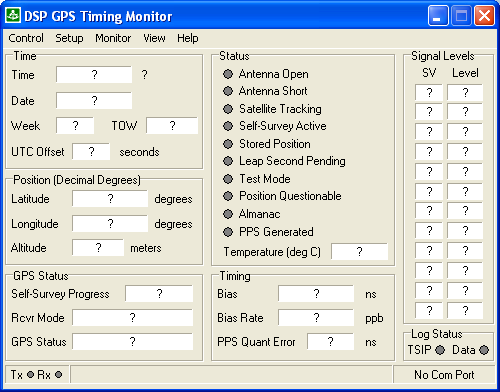
\includegraphics[scale=.5]{dspmon_main_nocom}
    \caption{Dit is het hoofdvenster van \dspmon als de COM poort niet
    goed staat.}
    \label{fig:dspmon_main_nocom}
\end{figure}

\begin{figure}
    \centering
    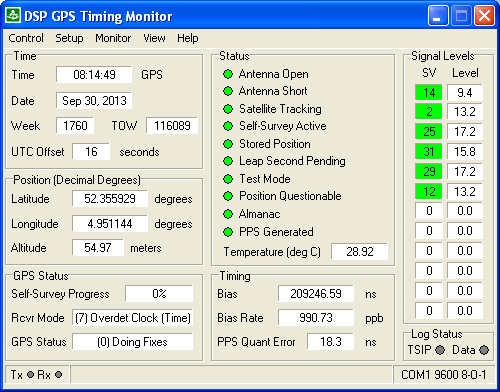
\includegraphics[scale=.5]{dspmon_main_com}
    \caption{Het hoofdvenster van \dspmon met goed herkende \gps, en
             signaal van 6 satellieten.}
    \label{fig:dspmon_main_com}
\end{figure}

Controleer alle instellingen van de \gps (onder het \emph{Setup} menu in
\dspmon) en zorg ervoor dat ze nauwkeurig overeenkomen met de
screenshots in de figuren \ref{fig:dspmon_receiver},
\ref{fig:dspmon_timing}, \ref{fig:dspmon_survey},
\ref{fig:dspmon_position} en \ref{fig:dspmon_options}. Onder de figuren
staat beschreven waar de instellingen belangrijk voor zijn. Deze
instellingen zijn in het programma te vinden onder het menu
\emph{Setup}. Als een instelling aangepast moet worden, druk dan op de
bijbehorende \emph{Set} knop (soms meerdere per scherm) om de
aanpassingen op te slaan en toe te passen.

Als de \gps antenne positie nog niet bepaald is moet deze met behulp van
de Self-Survey gevonden worden. De Self-Survey kan gestart worden via
het \emph{Control} menu. Start hier de Self-Survey (na deze ingesteld te hebben
zoals in \figref{fig:dspmon_survey}) en kom een dag later terug om het
instellen af te maken! Vergeet niet na het bepalen van de positie om in
de \hisparc \daq de \daq mode uit en weer aan te zetten om zo de nieuwe
positie door te geven. Bij het aanzetten van de \daq mode wordt namelijk
de configuratie van het meetstation verstuurd naar de server.

\begin{figure}
    \centering
    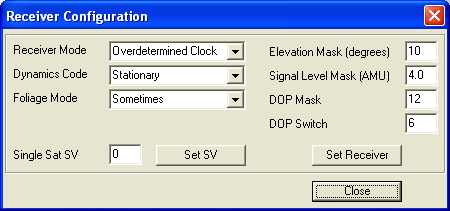
\includegraphics[scale=.5]{dspmon_receiver}
    \caption{In dit venster wordt gekozen hoe de \gps zich moet gedragen.
    Voor \hisparc is het van belang dat de tijd heel nauwkeurig bepaald
    wordt en staat de \gps vast. Vandaar dat we kiezen voor
    \emph{Overdetermined Clock} en \emph{Stationary}. De \emph{Elevation
    Mask} geeft aan dat satellieten minimaal \SI{10}{ degree} boven de
    grond moeten zijn om meegenomen te worden, omdat het signaal van
    lage satellieten eerder verstoord is door de atmosfeer.}
    \label{fig:dspmon_receiver}
\end{figure}

\begin{figure}
    \centering
    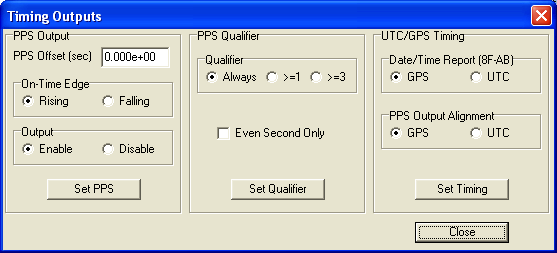
\includegraphics[scale=.5]{dspmon_timing}
    \caption{Hier worden de tijdsinstellingen gedaan. Het is zeer
    belangrijk om hier goed te controleren dat de \gps de \gps tijd
    geeft, en geen UTC-tijd.}
    \label{fig:dspmon_timing}
\end{figure}

\begin{figure}
    \centering
    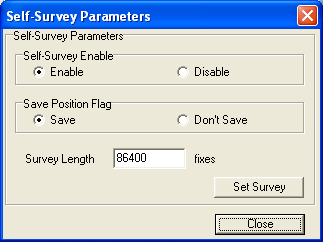
\includegraphics[scale=.5]{dspmon_survey}
    \caption{In dit venster worden instellingen voor de
             \emph{Self-Survey} gemaakt. De Self-Survey wordt gebruikt
             om de positie van de \gps te bepalen. Hierbij middelt de
             \gps over alle posities gemeten tijdens de Self-Survey. Het
             is belangrijk dat deze lang genoeg duurt, namelijk één dag
             (dus \SI{86400}{\second}). In paragraaf \ref{sec:gps} is
             uitgelegd dat de posities van de \gps satellieten zich
             iedere ongeveer iedere \SI{24}{uur} herhalen boven de aarde
             zich.}
    \label{fig:dspmon_survey}
\end{figure}
   
\begin{figure}
    \centering
    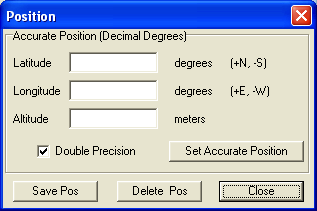
\includegraphics[scale=.5]{dspmon_position}
    \caption{Dit venster kan gebruikt worden om een eerste schatting van
    de positie in te vullen, maar let hier mee op dat deze niet wordt
    vastgezet als definitieve positie. Het is veiliger om deze
    instellingen leeg te houden en de \gps zelf zijn positie te laten
    bepalen door middel van de Self-Survey.}
    \label{fig:dspmon_position}
\end{figure}

\begin{figure}
    \centering
    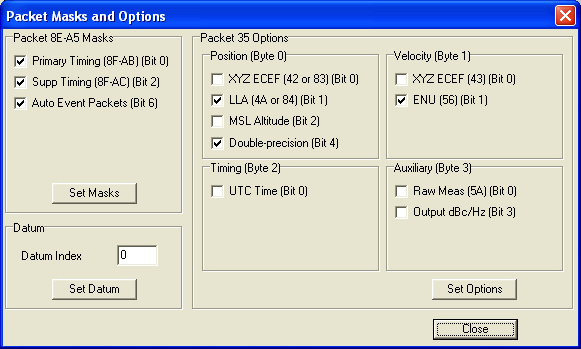
\includegraphics[scale=.5]{dspmon_options}
    \caption{De \gps kent vele opties waarvan een aantal door de \hisparc
    software worden gebruikt. Controleer deze vinkjes goed.}
    \label{fig:dspmon_options}
\end{figure}

Na het instellen van de \gps en het doorlopen van de Self-Survey is in
de \hisparc \daq als het goed is de \gps positie te zien en kan je in
het Satellites tabblad de signaal sterktes van de satellieten zien. Dit
is een grafiek waarin de kleur de sterkte van het signaal aangeeft, de
$y$-as het satelliet nummer en de $x$-as de tijd (tot 2 dagen in het
verleden). Na verloop van tijd zal er dus een grafiek zijn opgebouwd
waarin je goed kan zien hoe \gps signalen zich gedragen over het verloop
van de dag. In \figref{fig:hisparcdaq_satellites} is hier een voorbeeld
van te zien.

\begin{figure}
    \centering
    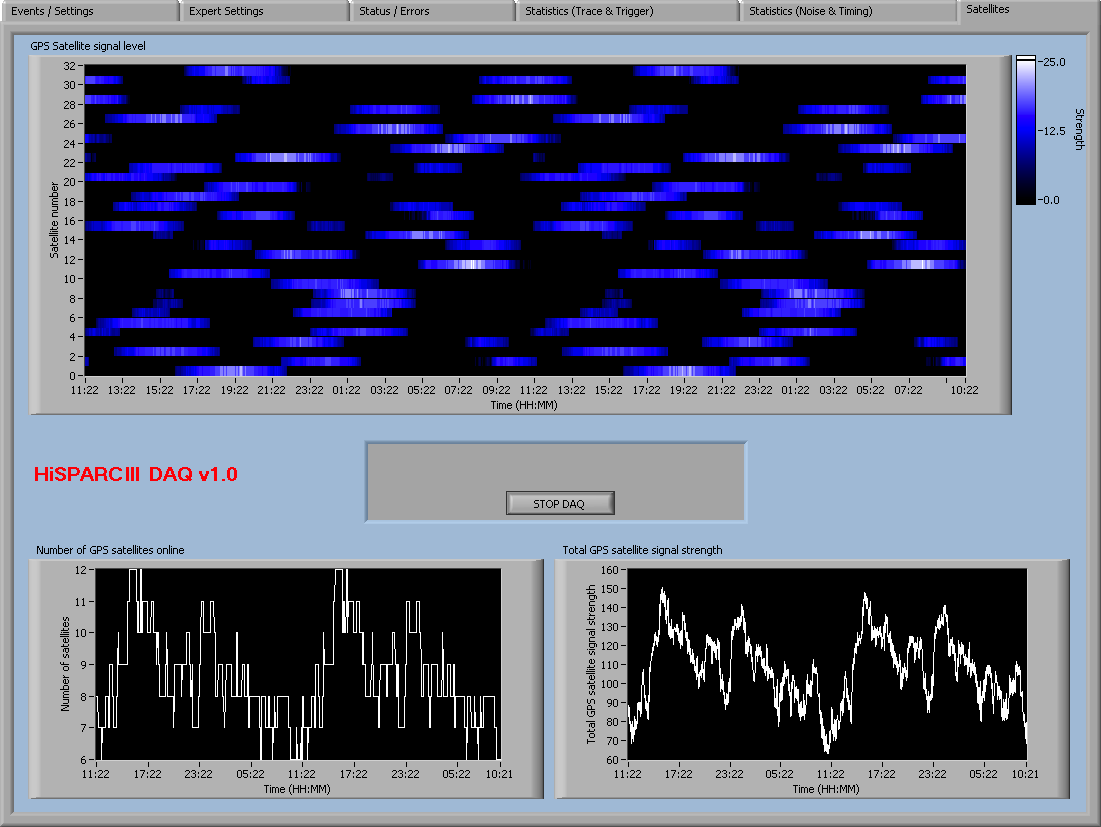
\includegraphics[scale=.4]{hisparcdaq_satellites}
    \caption{In de \hisparc \daq kan kan men een overzicht zien van de
    sterkte van de satelliet signalen. Hier is duidelijk te zien dat het
    signaal zich iedere 24 uur herhaald.}
    \label{fig:hisparcdaq_satellites}
\end{figure}

\begin{thebibliography}{9}
    \bibitem{gps2013gov} National Coordination Office (NCO), \emph{Basics
    of the GPS Technique: Observation Equations} (2013),\\
    \url{http://www.gps.gov/}.

    \bibitem{easton2006who} R. Easton, \emph{Who invented the Global
    Positioning System?} (2006),\\
    \url{http://www.thespacereview.com/article/626/1}.

    \bibitem{gent2003wet} R.H. van Gent, \emph{De wettelijke
    tijdregeling in Nederland} (2003--2009),\\
    \url{http://www.staff.science.uu.nl/~gent0113/wettijd/wettijd.htm}.

    \bibitem{software-software-doc} Het \hisparc team, \emph{\hisparc
    software documentatie} (2009--2012),\\
    \url{http://docs.hisparc.nl/station-software/doc/}.

    \bibitem{blewitt1997gps} G. Blewitt, \emph{Basics of the GPS
    Technique: Observation Equations} (1997),\\
    \url{http://www.nbmg.unr.edu/Staff/pdfs/Blewitt%20Basics%20of%20GPS.
    pdf}.

    \bibitem{ashby1997gen} N. Ashby, \emph{General relativity in the
    global positioning system} (1997),\\
    \url{http://www.phys.lsu.edu/mog/mog9/node9.html}.

    \bibitem{nist2013ces} R. Easton, \emph{NIST-F1 Cesium Fountain
    Atomic Clock} (2013),\\
    \url{http://www.nist.gov/pml/div688/grp50/primary-frequency-
    standards.cfm}.

    \bibitem{trimble2007res} Trimble, \emph{Resolution-T Data Sheet}
    (2007),\\
    \url{http://trl.trimble.com/docushare/dsweb/Get/Document-550777/}.
\end{thebibliography}

\end{document}
